\chapter{Technologie wykorzystane w aplikacji}
\label{chap4}
Poniższy rozdział opisuje wewnętrzną architekturę aplikacji. Zwraca uwagę na jej wielowarstwowy charakter. Dla każdej z warstw opisuje technologie, w których dana warstwa może być realizowana, zwracając szczególną uwagę na te, które zostały wybrane do jej faktycznej implementacji.

\section[Aplikacja w architekturze wielowarstwowej][Aplikacja w architekturze wielowarstwowej]{Aplikacja w architekturze wielowarstwowej}
Podział systemu na warstwy pozwala na ułatwienia w całym cyklu życia aplikacji. W szczególności zmniejsza koszty jego modyfikacji, gdyż wprowadzane zmiany ograniczają się zazwyczaj tylko do jednej warstwy. 

Najprostszym przykładem wielowarstwowej architektury aplikacji jest model typu klient-serwer. Wyróżnia on dwie warstwy:
\begin{itemize}
	\item klienta, stronę żądającą dostępu do jakiejś usługi bądź zasobu,
	\item serwera, stronę udostępniająca daną usługę lub zasób.
\end{itemize}
Architektura ta, dobrze sprawdzająca w małych systemach, zaczęła sprawiać problemy wraz z rozrastaniem się logik biznesowych aplikacji. Efektem tego było pojawienie się pojęć cienkiego i grubego klienta (ang. \textit{thin client} i \textit{fat client}) dla określenia technik umieszczających logikę biznesową po jednej lub po drugiej stronie.

Ostatecznie projektanci systemów wydzielili jeszcze jedną warstwę (odpowiedzialną za realizację logiki biznesowej), doprowadzając do powstania architektury trójwarstwowej. Wyróżnia ona następujące warstwy:
\begin{itemize}
	\item warstwę prezentacji widoczną dla klienta,
	\item warstwę aplikacji realizującą logikę biznesową,
	\item warstwę źródła danych.
\end{itemize}
Rysunek \ref{warstwy} przestawia ogólny schemat aplikacji trójwarstwowej.

\begin{figure}[tdh]
    \begin{center}
	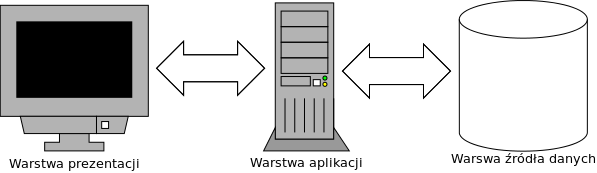
\includegraphics[scale=.7 ]{img/warstwy.png}
	\caption{Schemat komunikacji w architekturze trójwarstwowej}
	\label{warstwy}
    \end{center}
\end{figure}


\section[Warstwa prezentacji][Warstwa prezentacji]{Warstwa prezentacji}
Warstwa prezentacji stanowi interfejs miedzy użytkownikiem a systemem. Najbardziej podstawową implementacją tej warstwy jest terminal znakowy. Funkcje taką może pełnić również aplikacja okienkowa. W przypadku aplikacji webowych warstwa ta realizowana jest w przeglądarce internetowej za pomocą typowych technologii (takich jak HTML, CSS czy JavaScript).

\subsection[HTML][HTML]{HTML}
Podstawową technologią wykorzystywaną do tworzenia widoków aplikacji internetowych jest język znaczników HTML (ang. \textit{Hypertext Markup Language}). Najważniejszą jego zaletą jest przenośność. Zyskujemy dzięki temu niezależność interfejsu od środowiska użytkownika. Niestety sposób prezentacji wciąż jednak zależy (w niewielkim stopniu) od przeglądarki. Jednym z etapów projektu powinno więc być założenie jakie przeglądarki i od jakich wersji będą przez nas wspieranie. Należy też pamiętać, że standard HTML również podlega wersjonowaniu, co oznacza konieczność upewnienia się, czy wpierana przez nas przeglądarka obsługuje HTML w jego najnowszej - piątej wersji. W przeciwnym wypadku musimy ograniczyć się do funkcjonalności z edycji wcześniejszych.

Kolejną zaletą języka znaczników jest jego prostota. Dzięki niej nawet początkujący web-designerzy są w stanie szybko nauczyć się pisania kodu HTML.

Wadą języka HTML jest jego statyczność. Nawet najmniejsza zmiana na stronie wymaga ponownego wygenerowania żądania HTTP i przesłania go do serwera. Wpływa to negatywnie na responsywność aplikacji, szczególnie przy dużym obciążeniu. 
%Zdanie z SDI troche bez sensu ale mozna podrasowac
%Rozwiązaniem tego problemu są technologie takie jak np. AJAX, które generują kod wykonywany na poziomie przeglądarki, bez konieczności ponownego przesyłania żądania.

\subsection[CSS][CSS]{CSS}
W języku HTML możliwe jest wskazanie sposobu wyświetlania informacji. Zaleca się jednak, aby treść dokumentu była odseparowana od sposobu jej prezentacji. Umożliwiają to kaskadowe arkusze stylów (CCS). Pozwalają one na wydzielenie opisu sposobu prezentacji do specjalnych plików. Dzięki zastosowaniu tzw. selektorów możliwe jest zdefiniowanie jednolitego stylu dla całej aplikacji. Łatwiejsze staje się też zarządzanie jej wyglądem.

\subsection[JavaScript][JavaScript]{JavaScript}
JavaScript jest językiem skryptowym wykonywanym po stronie przeglądarki. Pozwala na częściowe ominięcie problemu statyczności dokumentu HTML. Zastosowanie JavaScriptu pozwala osiągnąć większą responsywność stron internetowych. Do typowych jego zastosowań należy obsługa dynamicznych elementów aplikacji (takich jak okna dialogowe) czy wstępna walidacja formularzy. Za pomocą JavaScriptu możemy też manipulować drzewem DOM dokumentu HTML.

\subsection[AJAX][AJAX]{AJAX}
\label{AJAX}
AJAX (ang. \textit{Asynchronous JavaScript and XML}) jest to wieloelementowa technologia pozwalająca na tworzenie kodu wykonującego się w całości po stronie klienta, bez konieczności przeładowywania stron. Daje ona możliwość wysyłania asynchronicznych zapytań do serwera. Pozwala to rozwiązać problem statyczności kodu HTML i daje możliwość tworzenia stron w pełni dynamicznych. Rozwiązanie to ma jednak kilka wad:
\begin{itemize}
	\item utrudnione zarządzanie historią w przeglądarce (mechanizmy pozwalające rozwiązać ten problem pojawiły dopiero w HTML5),
	\item brak możliwości indeksowania treści pobieranych za pomocą żądań AJAX. 
\end{itemize}
Oprócz wspomnianych wcześniej HTML'a, CSS'a i JavaScriptu w skład technologii AJAX wchodzą również:
\begin{itemize}
	\item XMLHttpRequest, klasa umożliwiająca asynchroniczne przesyłanie danych,
	\item XML (ang. \textit{Extensible Markup Language}), język znaczników pozwalający na przesyłanie informacji między klientem a serwerem (obecnie wykorzystuje się również nowsze typy danych np. JSON (ang. \textit{JavaScript Object Notation})).
\end{itemize}
Oczywiście korzystanie z AJAX'a nie zmusza programisty do rezygnacji z tradycyjnych żądań HTTP. Bardzo często można spotkać aplikacje, które większość swoich zapytań realizują synchronicznie, a asynchroniczne zapytania wykorzystują jedynie tam, gdzie ma znaczenie responsywność aplikacji.

\subsection[Dojo Toolkit][Dojo Toolkit]{Dojo Toolkit}
Dojo Toolkit jest zestawem narzędzi opartym na języku JavaScript. Składa się on z trzech podstawowych pakietów.

\subsubsection[dojo][dojo]{dojo}
Jest to główna część zestawu narzędziowego Dojo Toolkit. Zawiera ona najbardziej ogólne moduły pozwalające na komunikację z serwerem za pomocą technologii AJAX, manipulację drzewem DOM czy biblioteki służące do internacjonalizacji.

\subsubsection[dijit][dijit]{dijit}
Jest to zestaw standardowych komponentów interfejsu użytkownika tzw. widżetów (ang. \textit{widgets}) zbudowanych z wykorzystaniem narzędzi z pakietu dojo. Zawiera elementy takie jak np. okna dialogowe czy tooltipy. Na wyróżnienie zasługuje pakiet dijit.form zawierający elementy do budowy i walidacji formularzy.
 
\subsubsection[dojox][dojox]{dojox}
Jest to zestaw skomplikowanych widżetów i funkcji, zbudowanych na podstawie pakietów dojo i dijit. Pozwalają między innymi na tworzenie zaawansowanych efektów graficznych czy wizualizacje danych w postaci wykresów.
 
\section[Warstwa aplikacji][Warstwa aplikacji]{Warstwa aplikacji}
Warstwa aplikacji bywa też czasem nazywana warstwą logiki biznesowej. Jej podstawowym zadaniem jest pośredniczenie pomiędzy warstwą prezentacji a warstwą źródła danych. Odpowiada ona zarówno za odczyt i zapis danych, jak i za ich przekazywanie do wyświetlenia przez użytkownika. Realizuje przy tym często skomplikowaną logikę biznesową.

\subsection[Język programowania][Język programowania]{Język programowania}
Podstawową decyzją jaką musi dokonać projektant systemu jest wybór języka programowania. Determinuje on późniejszy wybór bibliotek, jakie zostaną użyte do tworzenia aplikacji. Ma też wpływ na komfort pracy deweloperów.

\subsubsection{Java}
Java jest językiem w pełni obiektowym. Do swojego działania potrzebuje maszyny wirtualnej, która jest dostępna dla większości (o ile nie dla wszystkich) obecnie spotykanych systemów operacyjnych. Zapewnia to przenośność napisanych w niej aplikacji. Istnieje mnóstwo bibliotek ułatwiających pracę w tym języku, z których większość jest dostępna bezpłatnie. Sam język jest rozwijany przez Oracle Corporation, który wykupił jego oryginalnego twórcę - Sun Microsystems.

\subsubsection{JEE}
Java Enterprise Edition jest rozszerzeniem standardowej platformy języka Java (tzw. Java Standard Edition). Przeznaczona jest ona do tworzenia aplikacji korporacyjnych. Podstawowym założeniem tej platformy jest osadzenie komponentów biznesowych na tzw. serwerze aplikacji (przykładem takiego serwera jest Apache Tomcat). Standardowym zadaniem serwera aplikacji jest praca na poziomie żądań HTTP (ang. \textit{Hypertext Transfer Protocol}), tzn. obsługa żądań oraz wysyłanie odpowiedzi. Zapewnia on także przechowywanie zmiennych sesyjnych 

\subsubsection{C\#}
Podobne funkcje jak Java może pełnić język C\# firmy Microsoft. Dzięki środowisku .NET nadaje się również do tworzenia aplikacji internetowych. Pomimo, iż twórca języka zapewnia o jego przenośności, nie działa on poprawnie na systemach spoza rodziny Windows. Na rynku jest sporo narzędzi ułatwiających programowanie w tym języku. Niestety, są one w większości płatne.

\subsection[Serwlety][Serwlety]{Serwlety}
Podstawowym komponentem realizującym założenia jakie stawia standard JEE jest serwlet. Wszystkie elementy, z których korzystamy tworząc aplikacje webowe (np. strony jsp) są zawsze ostatecznie kompilowane do postaci serwletów. Również frameworki służące do budowania aplikacji internetowych bazują na serwletach.

W ogólności, serwlet nie jest niczym innym jak klasą Javy implementująca interfejs Servlet. W praktyce spotyka się częściej serwlety dziedziczące z abstrakcyjnej klasy HttpServlet. Typowym działaniem takiego serwletu jest obsługa żądań HTTP oraz generowanie odpowiedzi. Zarówno żądanie jak i odpowiedź są oczywiście obudowane w odpowiednie klasy, ale o to dba już sam serwer aplikacji. Zadaniem serwera jest również przekazanie żądania do serwletu (wywołanie jego odpowiedniej metody) jak i odesłanie zwróconej przez serwlet odpowiedzi.

\subsection[ObjectLedge][ObjectLedge]{ObjectLedge}
ObjectLedge jest szkieletem aplikacyjnym (ang. \textit{framework}) bazującym na mechanizmie serwletów. Upraszcza on tworzenie aplikacji internetowych dostarczając szeregu narzędzi do realizacji typowych zadań. W jego skład wchodzi kilka modułów.

\subsubsection{Ledge Web}
Moduł Ledge Web służy do realizacji mechanizmu komunikacji użytkownika z systemem. Opiera się na wzorcu MVC (ang. \textit{Model-View-Controller}). Wzorzec ten polega on odseparowaniu od siebie elementów związanych z logiką biznesową oraz dostępem do danych od elementów związanych z widokiem. Najważniej cechą omawianego modułu jest potokowe przetwarzanie informacji. Programista sam określa sekwencje działań za pomocą tzw. zaworów (ang. \textit{Valve}). Do najważniejszych zadań zaworów należą:
\begin{itemize}
	\item obsługa akcji - zadań niemających bezpośredniego wpływu na widok, ale stanowiących efekt uboczny wykonania żądania,
	\item przygotowanie widoku - części widocznej dla użytkownika.
\end{itemize}
Typowym przykładem potoku jest podział zaworów na 3 klauzule try-catch-finally, gdzie w bloku try umieszczamy zawory odpowiedzialne m. in. za pobranie parametrów zapytania HTTP, obsługę akcji, czy przygotowanie widoku, w bloku catch zawory odpowiedzialne za obsługę sytuacji wyjątkowych (też przygotowujące widok informujący o zaistnieniu takiej sytuacji), zaś w klauzuli finally zawory odpowiadające za przesłanie odpowiedzi do użytkownika.

Obsługę akcji zapewnia zawór o nazwie ActionExecutorValve. Zadaniem programisty jest jedynie zdefiniowanie klasy określającej, co ma zostać wykonane w ramach akcji oraz umieszczenie jej w odpowiedniej strukturze katalogów. Za odnalezienie i wykonanie akcji odpowiada już mechanizm MVC.

Do obsługi widoków wykorzystywany jest zawór BuilderExecutorValve. Pozwala on na ich definiowanie za pomocą odpowiednich klas Javy oraz mechanizmu Velocity (opisanego w dalszej części rozdziału).

\subsubsection{Ledge Intake}
\label{intake}
Moduł ten pozwala na realizację dwóch podstawowych zadań:
\begin{itemize}
	\item konwersji formularzy wprowadzanych przez użytkownika na obiekty języka Java,
	\item walidacji wprowadzanych formularzy.
\end{itemize}
Pierwsze z nich realizowane jest przez zdefiniowanie powiązań pomiędzy polami formularza a właściwościami (ang. \textit{property}) obiektów javowych. Drugie z zadań odbywa się przez zdefiniowanie cech jakie powinny spełniać poszczególne pola formularza. Cechami takimi mogą być między innymi: wartość minimalna czy maksymalna,  format zapisu liczbowego, wyrażenie regularne lub informacja, czy dane pole jest wymagane. Dla każdej z tych cech możliwe jest zdefiniowanie komunikatów, jakie powinny być wyświetlane jeśli dana cecha nie jest spełniona. Do szczególnych zalet modułu Intake należy mocne wsparcie dla internacjonalizacji.

\subsubsection{Ledge Container}
Moduł ten pozwala na zarządzanie zależnościami pomiędzy komponentami programu poza jego kodem. Polega to na zdefiniowaniu klas oraz powiązań między nimi w specjalnym pliku xml. Dzięki temu zależności stają się dynamiczne tzn. nie są definiowane statycznie w momencie kompilacji, ale ustalane są dopiero w momencie wykonania. Pozwala to na zmianę zachowania programu bez konieczności jego rekompilacji (na przykład na zmianę klasy implementującej jakiś interfejs). Takie podejście nazywamy odwróceniem sterowania (ang. \textit{Inversion-of-Control}, w skrócie IoC). Dynamiczne powiązania obiektów możliwe są dzięki mechanizmowi wstrzykiwania zależności (ang. \textit{Dependency Injection}). LegdeContainer bazujący na narzędzi PicoContainer wykorzystuje wstrzykiwanie zależności przez konstruktor. Oznacza to, że wszystkie zależności danego obiektu powinny być argumentami jego konstruktora. Innym przykładem wstrzykiwania zależności jest np. wstrzykiwanie zależności przez metodę ustawiającą (ang. \textit{setter}) popularne w frameworku Spring. Do przechowywania obiektów służy tzw. Kontener. Odpowiada on m. in. za ich poprawną inicjalizację (ustalenie argumentów i przekazanie ich do konstruktora) na początku działania aplikacji.

\subsubsection{Ledge Security}
\label{security}
Moduł ten pozwala na realizację 2 podstawowych zadań stawianych systemom bezpieczeństwa: uwierzytelniania i autoryzacji.

\paragraph{Uwierzytelnianie} polega na sprawdzeniu tożsamości użytkownika, tzn. zweryfikowania czy użytkownik jest rzeczywiście tym, za kogo się podaje. Moduł bezpieczeństwa pozwala na uwierzytelnianie za pomocą nazwy użytkownika i hasła. Warto zaznaczyć, że hasła nie są przechowywane w postaci jawnej, ale w postaci ich funkcji skrótu (przykładem takiej funkcji jest MD5). Uniemożliwia to wejście w posiadanie haseł ani administratorom systemu ani też osobą, które w jakiś (być może niezgodny z prawem) sposób uzyskają dostęp do bazy danych. Oczywiście programista nie jest zmuszony do korzystania z tej postaci uwierzytelniania (wszystko zależy od tego, w jaki sposób zdefiniuje akcję logującą). Możliwe jest m. in. skorzystanie z zewnętrznego systemu służącego do identyfikacji takiego jak LDAP (ang. \textit{Lightweight Directory Access Protocol}, przykładem jego implementacji jest Active Directory firmy Microsoft).

\paragraph{Autoryzacja} polega na przydzieleniu (uwierzytelnionemu wcześniej) użytkownikowi uprawnień do wykonania określonych czynności na określonych obiektach. Mechanizm ten jest w ObjectLedge'u bardzo rozbudowany. Pozwalana on na dynamiczne tworzenie grup zasobów. Mogą być one powiązane z jakąś klasą obiektów, bądź z ich konkretnymi instancjami. W ramach grup użytkownikom przydzielane są role. Role zaś wiążą się z konkretnymi pozwoleniami (ang. \textit{permission}). Pozwolenia te określą dostęp do poszczególnych widoków, akcji oraz wywołań AJAX w ramach danej grupy zasobów.

\subsection[Apache Velocity][Apache Velocity]{Apache Velocity}
\label{velocity}
Velocity jest mechanizmem szablonów pozwalającym na szybkie tworzenie dokumentów. W przypadku aplikacji webowych są to zazwyczaj dokumenty HTML, co jednak nie jest regułą. Velocity jest też powszechnie wykorzystywane do tworzenia dokumentów w standardzie XML i jego pochodnych (np. XHTML czy VoiceXML). Najważniejszą cechą tego mechanizmu jest to, że został on w całości napisany w Javie. Pozwala to na odwoływanie się z poziomu kodu szablonów bezpośrednio do obiektów tego języka. Pozwala on również na definiowanie zmiennych, instrukcji warunkowych oraz pętli za pomocą odpowiednich makr, a także na dodawanie makr zdefiniowanych przez programistę.

\subsection[Spring Framework][Spring Framework]{Spring Framework}
Spring, podobnie jak ObjectLedge, jest szkieletem aplikacyjnym przeznaczonym dla platformy Java/JEE. Składa się on z kilku niezależnych modułów. Do najważniejszych z nich należą:
\begin{itemize}
	\item kontener IoC, 
	\item szablon programowania aspektowego,
	\item szablon dostępu do danych,
	\item szablon zarządzania transakcjami,
	\item szablon MVC,
	\item szablon bezpieczeństwa.
\end{itemize}
Niestety, duża ilość komponentów wpływa negatywnie na wydajność. Powoduje to powolną migrację programistów w stronę innych frameworków. Mimo to, Spring jest ciągle najpopularniejszym narzędziem tego typu.

%\subsection[Java Server Pages][Java Server Pages]{Java Server Pages}
%TODO jako alternatywa dla Velocity

\subsection[JDBC][JDBC]{JDBC}
JDBC (ang. \textit{Java DataBase Connectivity}, częśc platformy Java Standard Edition) jest interfejsem pozwalającym na wykonywanie zapytań SQL z poziomu języka Java. Do poprawnego działania wymaga sterownika bazy danych, z którą ma współpracować. Niestety korzystanie z niego bezpośrednio w aplikacji jest uciążliwe, a stąd rzadko spotykane. Służy jednak jako podstawa do bardziej zaawansowanych narzędzi realizujących dostęp do warstwy danych. Najprostszym przykładem takiego narzędzia jest JdbcTemplate z frameworka Spring. Z JDBC korzystają również narzędzia służące do mapowania obiektowo-relacyjnego (ang. \textit{object-relational mapping}, w skrócie ORM) takie jak Hibernate.

\subsection[Hibernate][Hibernate]{Hibernate}
\label{hibernate}
Hibernate jest obecnie najpopularniejszym frameworkiem pozwalającym na implementację warstwy dostępu do danych (ang. \textit{persistence layer}). Został on stworzony z myślą o języku Java, istnieje jednak jego wersja dla środowiska .NET (tzw. NHibernate).

Podstawowym zadaniem jakie spełnia Hibernate jest odwzorowanie struktury obiektów języka Java na relacyjną bazę danych, zwane mapowaniem obiektowo-relacyjnym. Odwzorowania tego można dokonać na dwa sposoby:
\begin{itemize}
	\item z wykorzystaniem plików hbm.xml,
	\item za pomocą adnotacji JPA (Java Persistence API).
\end{itemize}

Pliki hbm.xml (ang. \textit{Hibernate Mapping files}) są podstawowym sposobem realizacji mapowania obiektowo-relacyjnego w Hibernate. Mają one format dokumentów xml zawierających informacje o sposobie, w jaki dane z tabel relacyjnych mają być tłumaczone na obiekty domenowe. Do najważniejszych z nich należą: nazwa tabeli oraz kwalifikowana nazwa klasy, informacje o kluczu głównym, nazwy kolumn tabeli i właściwości (niekoniecznie pól) klasy czy  informacje o relacjach z innymi tabelami (również odwzorowywanymi w strukturze obiektowej). Nie ma ograniczenia na liczbę klas, które można zmapować za pomocą jednego pliku, zaleca się jednak, aby mapowanie każdej klasy znajdowało się w osobnym dokumencie. Istnieją narzędzia pozwalające na automatyczną generację klas domenowych oraz plików hbm.xml na podstawie struktury bazy danych. Jednym z nich jest Hibernate Tools, będący częścią projektu Hibernate.

Java Persistence API jest oficjalnym standardem języka Java służącym do mapowania obiektowo-relacyjnego. Standard ten jest implementowany nie tylko przez Hibernate, ale też przez inne ORM-y, co umożliwia zmianę narzędzia bez konieczności przebudowy dużej części aplikacji. Założeniem JPA jest wykorzystanie specjalnie przygotowanych adnotacji języka Java bezpośrednio w kodzie klas, które mają być odwzorowane na tabele. Pozwala to zwiększyć czytelność kodu, sprawiając, że zarówno klasa jak i jej mapowanie znajdują się w jednym pliku. Wadą tego rozwiązania są mniejsze możliwości niż plików hbm.xml. Pamiętać także należy, że adnotacje pojawiły się w Javie dopiero w wersji 1.5, co może okazać się kłopotliwe w przypadku korzystania ze starszych wersji oprogramowania.

Hinernate oferuje również bazujący na SQL język - HQL (ang. \textit{Hibernate Query Language }). Pozwala on na tworzenie zapytań z wykorzystaniem obiektów domenowych. Zaletą tego rozwiązania jest to, że niewielkie zmiany w bazie danych (np. zmiana nazwy tabeli bądź kolumny) nie muszą oznaczać konieczności zmian zapytań HQL.

\section[Warstwa źródła danych][Warstwa źródła danych]{Warstwa źródła danych}
Najważniejszym elementem aplikacji jest system zarządzania bazą danych (ang. \textit{Database Management System}, w skrócie DBMS). Jako jedyny jest prawie niemożliwy do wymiany. Decyzja o jego wyborze powinna być starannie przemyślana, gdyż może stanowić o przyszłym powodzeniu lub klęsce całego systemu.

\subsection[Oracle Database 11g Express Edition][Oracle Database 11g Express Edition]{Oracle Database 11g Express Edition} 
Niekwestionowanym liderem rynku systemów zarządzania bazą danych jest firma Oracle ze swoim produktem zwanym Oracle Database. Niestety większość jego wersji (takich jak np. Oracle Database Enterprise Edition) jest płatna. Bezpłatnie dostępna jest jedynie wersja Express Edition oznaczona numerem 11g (najnowsza edycja 12c dostępna jest tylko w wersjach płatnych).  Posiada ona jednak istotne ograniczenia. Do podstawowych z nich należą:
\begin{itemize}
	\item wykorzystanie mocy obliczeniowej co najwyżej jednego procesora,
	\item ograniczenie wykorzystania pamięci RAM do 1GB,
	\item ograniczenie rozmiaru bazy danych do 11GB,
	\item brak wsparcia technicznego.
\end{itemize}

\subsection[MySQL][MySQL]{MySQL} 
MySQL jest prawdopodobnie najpopularniejszym darmowym systemem zarządzania bazą danych. Szczególnie chętnie bywa łączony z technologiami takimi jak PHP, służąc do budowy stron internetowych oraz prostych aplikacji webowych. W śród deweloperów krąży jednak wiele negatywnych opinii na jego temat. Od 2010 roku jest rozwijany przez firmę Oracle.

\subsection[PostgreSQL][PostgreSQL]{PostgreSQL} 
PostgreSQL, zwany też po prostu Postgres, jest bardzo zaawansowanym systemem zarządzania bazą dodanych. Jest on następcą nieistniejącego już systemu o nazwie Ingres. Rozpowszechniany jest na zasadzie wolnego oprogramowania na licencji zwanej PostgreSQL, podobnej do licencji BSD. Do jego najważniejszych cech należą:
\begin{itemize}
	\item rozbudowany język proceduralny PL/pgSQL (podobny do PL/SQL używanego w bazach Oracle),
	\item zgodność ze standardem SQL:2008 (implementuje też większość nowszego standardu SQL:2011),
	\item rozszerzona definicja typów (w porównaniu do standardu SQL),
	\item wysoka wydajność (m. in. dzięki zastosowaniu mechanizmu MVCC (ang. \textit{Multiversion Concurrency Control}) do zarządzania transakcjami),
	\item brak ograniczeń na rozmiar bazy danych(istnieją czysto techniczne ograniczenia na wielkość niektórych elementów w bazie, ale są one liczone w terabajtach i nie powinny mieć wpływu na działanie aplikacji),
	\item stabilność działania,
	\item dostępność na większość używanych obecnie systemów operacyjnych (Wiele dystrybucji likuksa zawiera pakiety umożliwiające instalację bazy PostgreSQL, znajdują się one m. in. w repozytorium popularnej dystrybucji Ubuntu),
	\item bogata dokumentacja.
\end{itemize}
Wszystkie te czynniki czynią Postgres jednym z trzech (obok wspomnianego wcześniej MySQL i Firebird) najpopularniejszych systemów zarządzania bazą danych dostępnych za darmo. W 2012 roku został odznaczony tytułem Linux New Media Award for Best Open Source Database.

\section[Narzędzia wspomagające tworzenie aplikacji][Narzędzia wspomagające tworzenie aplikacji]{Narzędzia wspomagające tworzenie aplikacji}

\subsection[Eclipse][Eclipse]{Eclipse}
Eclipse jest popularnym zintegrowanym środowiskiem programistycznym (ang. \textit{Integrated Development Environment}, IDE). Mimo, iż jest ono przeznaczone głównie do tworzenia programów w języku Java, możliwe jest jego wykorzystanie do programowania w różnych językach. Zapewnia to mechanizm wtyczek (ang. \textit{plugin}). Pozwalają one na dowolne rozszerzanie jego funkcjonalności. Umożliwiają one nie tylko wspomaganie programowania w danym języku, ale również tworzenie GUI, modelowanie w UML, współpracę z bazami danych czy serwerami aplikacji. Przykładem aplikacji zbudowanej z platformy Eclipse oraz odpowiedniego zestawu wtyczek jest Rational Software Architect firmy IBM.

\subsection[Maven][Maven]{Maven}
Maven jest narzędziem automatyzującym proces budowy oprogramowania. Budowanie to odbywa się na podstawie opisu projektu zawartego w specjalnym pliku o nazwie pom.xml. Plik taki zawiera najważniejsze informacje o projekcie oraz sposobie jego budowania. Nie zawiera natomiast (w przeciwieństwie np. do Anta) szczegółowego opisu kroków, w jakich miałby przebiegać proces budowy aplikacji. Ważnym elementem takiego pliku są tzw. zależności (ang. \textit{dependency}) - biblioteki wykorzystywane przez tworzoną aplikację. Są one automatycznie pobierane ze zdalnego repozytorium Mavena (bądź innego wskazanego w pliku pom.xml), a następnie umieszczane w lokalnym repozytorium na komputerze programisty. Budowanie aplikacji odbywa się przez osiągnięcie wybranego przez programistę celu. Do najważniejszych z nich należą:
\begin{itemize}
	\item compile - kompilacja kodu źródłowego,
	\item test - uruchomienie testów jednostkowych,
	\item package - budowa tzw. paczki najczęściej w postaci archiwum JAR lub WAR,
	\item install - umieszczenie paczki w lokalnym repozytorium,
	\item deploy - umieszczenie paczki w zdalnej lokalizacji np. na serwerze aplikacji.
\end{itemize}
Wymienione cele są, częścią tzw. głównego cyklu życia projektu. Oznacza to, że w osiągnięcie każdego z nich powinno być poprzedzone realizacją celów znajdujących się na wyższych pozycjach listy.

